% supplement_main.tex
% Supplementary Material for:
% Solis-Lemus et al. | PLOS Computational Biology | PCOMPBIOL-D-25-02375
%
% Compile: ./rerunpdf.sh supplement_main
% Final:   ./rerunpdf.sh -f supplement_main
% -------------------------------------------------------------------------

\documentclass[10pt,letterpaper]{article}

\usepackage[top=1in,left=1in,right=1in,bottom=1in]{geometry}
\usepackage{cite}

% draft/final toggle — must be defined BEFORE % preamble_shared.tex
% Shared packages and macros for plos_latex_template.tex and supplement_main.tex
% DO NOT add layout/geometry/header packages here — those are file-specific.
% -------------------------------------------------------------------------

% Core math
\usepackage{amsmath,amssymb}

% Additional characters
\usepackage{textcomp,marvosym}

\iffinal
    \usepackage[final,commentmarkup=footnote]{changes}  % use mode draft to show changes
\else
    \usepackage[draft,commentmarkup=footnote]{changes}  % use mode draft to show changes
\fi
\definechangesauthor[name={Reviewer 1}, color=blue]{R1}
\definechangesauthor[name={Reviewer 2}, color=orange]{R2}
\definechangesauthor[name={Reviewer 3}, color=teal]{R3}
\definechangesauthor[name={Multiple Reviewers}, color=magenta]{MR}
\definechangesauthor[name={Editor}, color=brown]{ED}


% Hyperlinks (nameref required for SI cross-references)
\usepackage{nameref,hyperref}

% Color (table shading)
\usepackage[table]{xcolor}

% Table utilities
\usepackage{array}
\usepackage{booktabs}

% Thick rule helpers (used in main manuscript tables)
\newcolumntype{+}{!{\vrule width 2pt}}
\newlength\savedwidth
\newcommand\thickcline[1]{%
  \noalign{\global\savedwidth\arrayrulewidth\global\arrayrulewidth 2pt}%
  \cline{#1}%
  \noalign{\vskip\arrayrulewidth}%
  \noalign{\global\arrayrulewidth\savedwidth}%
}
\newcommand\thickhline{%
  \noalign{\global\savedwidth\arrayrulewidth\global\arrayrulewidth 2pt}%
  \hline
  \noalign{\global\arrayrulewidth\savedwidth}%
}

% -------------------------------------------------------------------------
% SHARED MACROS
% -------------------------------------------------------------------------

% Simulation output symbols
\newcommand{\TAT}[1]{\ensuremath{\mathrm{TAT}_{#1}}}
\newcommand{\VOL}[1]{\ensuremath{\mathrm{Vol}_{#1}}}
\newcommand{\deltaVol}[1]{\ensuremath{\Delta \mathrm{Vol}_{#1}}}
\newcommand{\deltaVolNorm}[1]{\ensuremath{\mathcal{V}_{#1}}}

% Anatomical abbreviations
\newcommand{\LV}{LV}
\newcommand{\RV}{RV}
\newcommand{\LA}{LA}
\newcommand{\RA}{RA}
\newcommand{\SAN}{SAN}
\newcommand{\UKBB}{UKBB}

% Clinical group abbreviations
\newcommand{\Ctl}{$C$}
\newcommand{\HF}{$HF$}
\newcommand{\HFN}{$HF_N$}
\newcommand{\HFW}{$HF_W$}
\newif\iffinal
\finalfalse

% -------------------------------------------------------------------------
% SHARED PACKAGES AND MACROS
% -------------------------------------------------------------------------
% preamble_shared.tex
% Shared packages and macros for plos_latex_template.tex and supplement_main.tex
% DO NOT add layout/geometry/header packages here — those are file-specific.
% -------------------------------------------------------------------------

% Core math
\usepackage{amsmath,amssymb}

% Additional characters
\usepackage{textcomp,marvosym}

\iffinal
    \usepackage[final,commentmarkup=footnote]{changes}  % use mode draft to show changes
\else
    \usepackage[draft,commentmarkup=footnote]{changes}  % use mode draft to show changes
\fi
\definechangesauthor[name={Reviewer 1}, color=blue]{R1}
\definechangesauthor[name={Reviewer 2}, color=orange]{R2}
\definechangesauthor[name={Reviewer 3}, color=teal]{R3}
\definechangesauthor[name={Multiple Reviewers}, color=magenta]{MR}
\definechangesauthor[name={Editor}, color=brown]{ED}


% Hyperlinks (nameref required for SI cross-references)
\usepackage{nameref,hyperref}

% Color (table shading)
\usepackage[table]{xcolor}

% Table utilities
\usepackage{array}
\usepackage{booktabs}

% Thick rule helpers (used in main manuscript tables)
\newcolumntype{+}{!{\vrule width 2pt}}
\newlength\savedwidth
\newcommand\thickcline[1]{%
  \noalign{\global\savedwidth\arrayrulewidth\global\arrayrulewidth 2pt}%
  \cline{#1}%
  \noalign{\vskip\arrayrulewidth}%
  \noalign{\global\arrayrulewidth\savedwidth}%
}
\newcommand\thickhline{%
  \noalign{\global\savedwidth\arrayrulewidth\global\arrayrulewidth 2pt}%
  \hline
  \noalign{\global\arrayrulewidth\savedwidth}%
}

% -------------------------------------------------------------------------
% SHARED MACROS
% -------------------------------------------------------------------------

% Simulation output symbols
\newcommand{\TAT}[1]{\ensuremath{\mathrm{TAT}_{#1}}}
\newcommand{\VOL}[1]{\ensuremath{\mathrm{Vol}_{#1}}}
\newcommand{\deltaVol}[1]{\ensuremath{\Delta \mathrm{Vol}_{#1}}}
\newcommand{\deltaVolNorm}[1]{\ensuremath{\mathcal{V}_{#1}}}

% Anatomical abbreviations
\newcommand{\LV}{LV}
\newcommand{\RV}{RV}
\newcommand{\LA}{LA}
\newcommand{\RA}{RA}
\newcommand{\SAN}{SAN}
\newcommand{\UKBB}{UKBB}

% Clinical group abbreviations
\newcommand{\Ctl}{$C$}
\newcommand{\HF}{$HF$}
\newcommand{\HFN}{$HF_N$}
\newcommand{\HFW}{$HF_W$}

% -------------------------------------------------------------------------
% SUPPLEMENT-SPECIFIC LAYOUT
% -------------------------------------------------------------------------

% S-numbered figures and tables
\setcounter{figure}{0}
\renewcommand{\thefigure}{S\arabic{figure}}
\setcounter{table}{0}
\renewcommand{\thetable}{S\arabic{table}}

% Sections as S1, S2... (optional — comment out if you prefer plain numbering)
\renewcommand{\thesection}{S\arabic{section}}

% Captions
\usepackage[aboveskip=1pt,labelfont=bf,labelsep=period,
            justification=raggedright,singlelinecheck=off]{caption}
\renewcommand{\figurename}{S Fig}
\renewcommand{\tablename}{S Table}

% Header/footer
\usepackage{lastpage,fancyhdr}
\pagestyle{fancy}
\fancyhf{}
\rfoot{\thepage/\pageref{LastPage}}
\lfoot{Solis-Lemus et al. --- Supplementary Material}
\renewcommand{\headrulewidth}{0pt}
\renewcommand{\footrule}{\hrule height 1pt \vspace{2mm}}

% Line numbers (comment out if not wanted in supplement)
\usepackage[right]{lineno}

% Ligatures
\usepackage[nopatch=eqnum]{microtype}
\DisableLigatures[f]{encoding = *, family = * }

% Bibliography
\bibliographystyle{plos2025}
\makeatletter
\renewcommand{\@biblabel}[1]{\quad#1.}
\makeatother

% Text layout
\raggedright
\setlength{\parindent}{0.5cm}

% =========================================================================
\begin{document}

\begin{center}
    {\Large\textbf{Supporting Information}}\\[6pt]
    {\normalsize Solis-Lemus et al. | \textit{PLOS Computational Biology} |
    PCOMPBIOL-D-25-02375}
\end{center}

\bigskip
\linenumbers

% -------------------------------------------------------------------------
% S1 FIGURE: TAT-QRS Correlation
% -------------------------------------------------------------------------
\begin{figure}[htbp]
    \centering
    %
\includegraphics[width=\textwidth]{../pics/sp1_supp_tat_qrs_stratified.pdf}
    \caption{
        \textbf{Correlation between simulated ventricular total activation time
        (\TAT{V}) and recorded ECG QRS duration, stratified by condition.}
        In \Ctl{} hearts (blue, $n=17$), \TAT{V} showed a strong positive
        correlation with QRS duration (Pearson $r = 0.649$, $p = 0.005$),
        indicating that anatomical variability alone can predict conduction time
        in healthy myocardium when using uniform electrophysiological parameters.
        In \HF{} patients (red, $n=16$), no correlation was observed
        ($r = -0.127$, $p = 0.64$), reflecting that pathological conduction
        delays (fibrosis, scar, conduction blocks) are not captured by anatomy
        alone and would require patient-specific tissue property calibration.
    }
    \label{fig:s1-tat-qrs}
\end{figure}


% -------------------------------------------------------------------------
% S2 TABLE: Geometric Characteristics
% -------------------------------------------------------------------------
\begin{table}[htbp]
\centering
\caption{
    \textbf{Geometric characteristics stratified by sex and heart failure status.}
    Mean $\pm$ SD reported for age (years), chamber volumes (mL), and total mesh
    elements (millions). \HF{} patients showed increased chamber volumes across
    all chambers, particularly pronounced in males. Mesh element counts scaled
    with anatomical size, reflecting the adaptive meshing algorithm.
}
\begin{tabular}{lccccccr}
\toprule
\textbf{Group} & $n$ & \textbf{Age (yr)} &
    $\VOL{\LV}$ \textbf{(mL)} & $\VOL{\RV}$ \textbf{(mL)} &
    $\VOL{\LA}$ \textbf{(mL)} & $\VOL{\RA}$ \textbf{(mL)} &
    \textbf{Elements ($\times 10^6$)} \\
\midrule
Male \Ctl   & 13 & $47.2 \pm 12.0$ & $179.6 \pm 36.3$ & $188.7 \pm 25.7$
            & $93.9 \pm 27.9$  & $100.7 \pm 16.9$ & $2.33 \pm 0.35$ \\
Male \HF    & 12 & $60.1 \pm 16.1$ & $289.1 \pm 88.1$ & $227.6 \pm 60.2$
            & $140.5 \pm 58.9$ & $138.2 \pm 67.7$ & $2.95 \pm 0.59$ \\
Female \Ctl & 13 & $49.5 \pm  9.8$ & $139.7 \pm 32.2$ & $139.7 \pm 34.8$
            & $79.6 \pm 19.4$  & $86.3 \pm 32.3$  & $1.91 \pm 0.28$ \\
Female \HF  & 12 & $60.1 \pm  9.0$ & $183.0 \pm 60.0$ & $136.7 \pm 30.8$
            & $104.9 \pm 57.4$ & $100.0 \pm 47.3$ & $2.17 \pm 0.38$ \\
\bottomrule
\end{tabular}
\label{tab:s2-geometric-characteristics}
\end{table}


% -------------------------------------------------------------------------
% S3 FIGURE: Correlation Heatmap
% -------------------------------------------------------------------------
\begin{figure}[htbp]
    \centering
    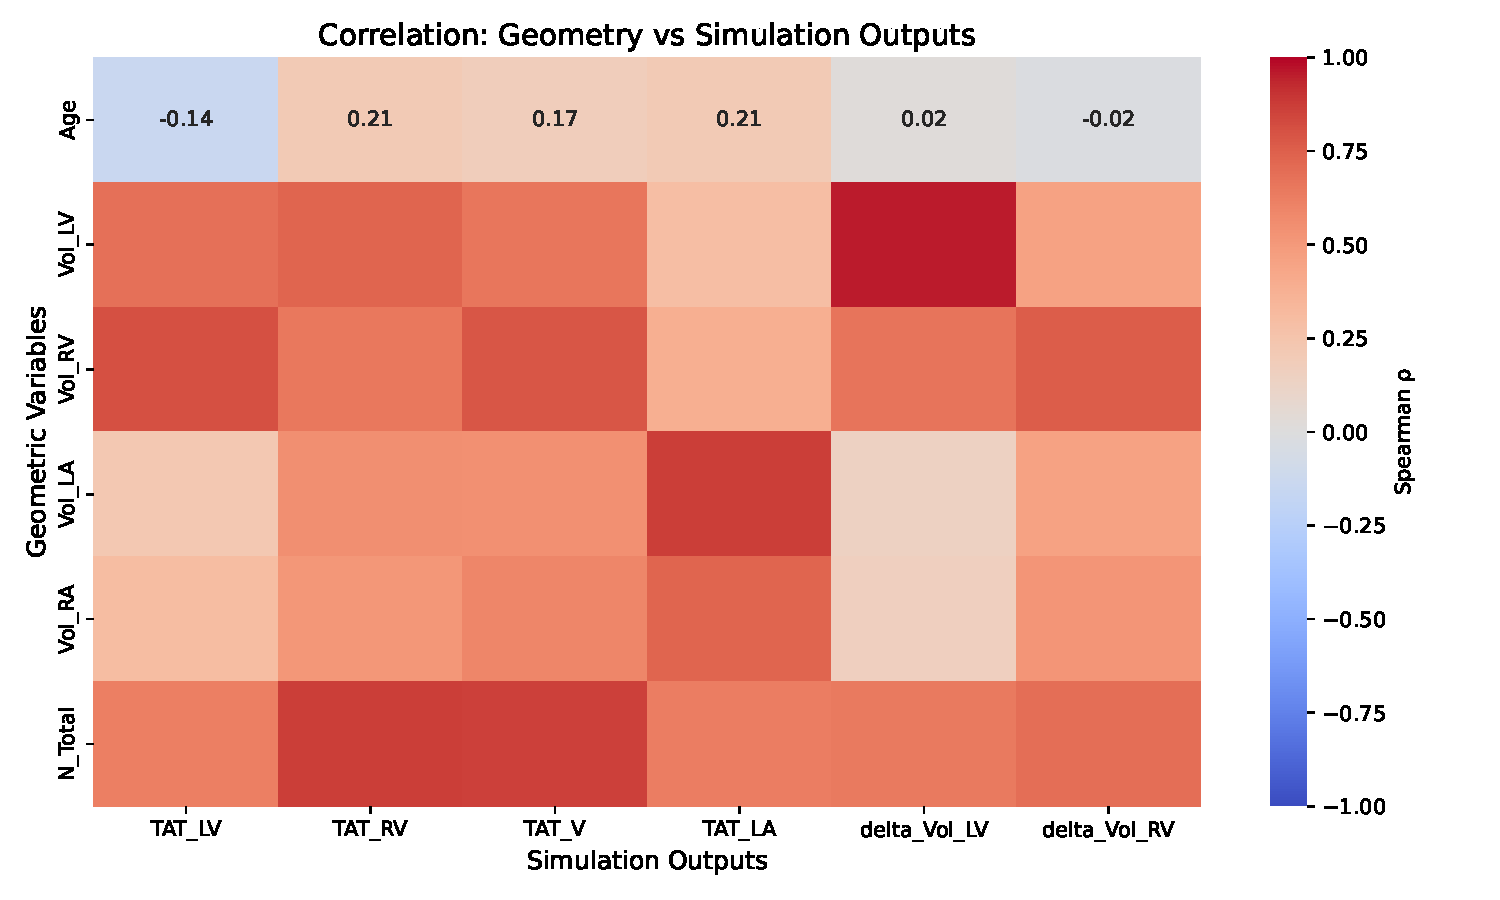
\includegraphics[width=\textwidth]{pics/sp2_correlation_heatmap.pdf}
    \caption{
        \textbf{Correlation matrix between geometric variables and simulation outputs.}
        Spearman correlation coefficients ($\rho$) shown for relationships between
        geometric metrics (chamber volumes, myocardial wall volume, age) and simulation
        outputs (activation times, volume changes). Strong positive correlations
        (red) indicate that geometric variables predict functional outcomes under
        standardised parameters. All correlations shown are statistically
        significant ($p < 0.05$).
}
    \label{fig:s3-correlation-heatmap}
\end{figure}


% -------------------------------------------------------------------------
% S4 TABLE: CGAL Parameters
% -------------------------------------------------------------------------
\input{sections/supp/s4_cgal_params}

% -------------------------------------------------------------------------
% S5 TABLE: 37-Label Specification
% -------------------------------------------------------------------------
% TODO: Fill in the 37 label IDs, names, and types from the CEMRG Heartbuilder
% label specification (see strocchi2020_cohort / strocchi2020_simulating).
% The structure types and categories below are derived from the methods section
% but the integer label IDs must be added before submission.
%
% Known structure categories (from Methods Section 3.1.1):
%   Blood pools:    LV, RV, LA, RA, Aorta, Pulmonary artery,
%                   LA pulmonary veins (sup/inf), RA pulmonary veins (sup/inf),
%                   LA appendage, Superior vena cava, Inferior vena cava
%   Myocardium:     LV, RV (3.5 mm thickness), LA, RA, Aortic wall, PA wall
%   Valve planes:   Mitral, Tricuspid, Aortic, Pulmonary
%   Vein rings:     Pulmonary vein rings, Vena cava rings

\subsection*{Mesh Label Specification}

The post-processing stage of the CEMRG Heartbuilder pipeline increases the
initial 10-label segmentation to 37 labels
(Figure~\ref{fig:methods-segmentation}c), following the standard introduced
by~\cite{strocchi2020_cohort,strocchi2020_simulating}. Labels encode
anatomical structures required for assigning tissue-specific electrophysiology
and mechanics model parameters during simulation setup.

\begin{table}[htbp]
\centering
\caption{
    \textbf{Complete list of 37 anatomical labels.}
    Labels are assigned during the post-processing stage of the segmentation
    pipeline. Structure types: BP = blood pool, Myo = myocardium,
    VP = valve plane, Ring = vein/artery ring. 
}
\begin{tabular}{clll}
\toprule
\textbf{Label ID} & \textbf{Structure name} & \textbf{Chamber} & \textbf{Type} \\
\midrule
1    & Left ventricular blood pool   & \LV & BP  \\
2    & Left ventricular myocardium   & \LV & Myo \\
3    & Right ventricular blood pool  & \RV & BP  \\
4    & Left atrial blood pool        & \LA & BP  \\
5    & Right atrial blood pool       & \RA & BP  \\
6    & Aortic blood pool             & ---  & BP  \\
7    & Pulmonary artery blood pool   & ---  & BP  \\
8    & Left superior pulmonary vein  & \LA & BP  \\
9    & Left inferior pulmonary vein  & \LA & BP  \\
10   & Right superior pulmonary vein & \RA & BP  \\
11   & Right inferior pulmonary vein & \RA & BP  \\
12   & Left atrial appendage         & \LA & BP  \\
13   & Superior vena cava            & \RA & BP  \\
14   & Inferior vena cava            & \RA & BP  \\
103    & Right ventricular myocardium  & \RV & Myo \\
104    & Left atrial myocardium        & \LA & Myo \\
105    & Right atrial myocardium       & \RA & Myo \\
106    & Aortic wall                   & ---  & Myo \\
107    & Pulmonary artery wall         & ---  & Myo \\
201    & Mitral valve plane            & \LV/\LA & VP \\
202    & Tricuspid valve plane         & \RV/\RA & VP \\
203    & Aortic valve plane            & \LV & VP  \\
204    & Pulmonary valve plane         & \RV & VP  \\
205   & Left superior pulmonary vein plane & \LA & VP  \\
206   & Left inferior pulmonary vein plane & \LA & VP  \\
207   & Right superior pulmonary vein plane & \LA & VP  \\
208   & Right inferior pulmonary vein plane & \LA & VP  \\
209   & Left atrial appendage plane & \LA & VP \\
210   & Superior vena cava plane & \RA & VP  \\
211   & Inferior vena cava plane  & \RA & VP \\
221    & Left superior pulmonary vein ring     & \LA & Ring \\
222    & Left inferior pulmonary vein ring     & \LA  & Ring \\
223    & Right superior pulmonary vein ring    & \LA  & Ring \\
224   & Right inferior pulmonary vein ring    & \LA & Ring \\
225    & Left atrial appendage vein ring   & \LA & Ring \\
226    & Superior vena cava vein ring  & \RA & Ring  \\
227    & Inferior vena cava vein ring  & \RA & Ring  \\
\bottomrule
\end{tabular}
\label{tab:s5-labels}
\end{table}


% -------------------------------------------------------------------------
% S6 METHODS: Boundary Conditions
% -------------------------------------------------------------------------
\input{sections/supp/s6_boundary_conditions}

% -------------------------------------------------------------------------
% S7 TABLE (optional): Per-model Mesh Quality Statistics
% -------------------------------------------------------------------------
% \input{sections/supp/s7_mesh_quality}

\nolinenumbers

\bibliography{myrefs}

\end{document}